\documentclass[uplatex, a4paper, 12pt, openany, oneside]{jsbook}

\usepackage[dvipdfmx]{graphicx}
\usepackage[dvipdfmx]{color}
\usepackage[dvipdfmx, bookmarks=true, setpagesize=false, hidelinks]{hyperref}
\usepackage{pxjahyper}

\usepackage{thesis}
\usepackage{here}
\usepackage{url}


\thesis{インテリジェントロボットモーション}
\title{
  \centering
    \scalebox{1.0}{ラグランジュ法}\\
    \vspace{-0.3zh}
    \scalebox{0.7}{Lagrangian Formulation}
    \vspace{-0.6zh}
}
\setlength{\textwidth}{\fullwidth}
\setlength{\evensidemargin}{\oddsidemargin}

\date{\today}
\vspace{-15.0zh}
\teacher{林原 靖男 教授}
\vspace{-15.0zh}
\organization{千葉工業大学 先進工学部 未来ロボティクス学科}
\author{20C1102 馬場 琉生}
\vspace{-15zh}

\renewcommand{\baselinestretch}{1.2}
\begin{document}

%% Front Matter
\frontmatter{}
%
\maketitle
%
%!TEX root = ../thesis.tex
\chapter*{概要}
\thispagestyle{empty}
%
\begin{center}
  \scalebox{1.5}{ラグランジュ法}\\
\end{center}
\vspace{1.0zh}
%
 三次元空間で運動する場合,並進運動と回転運動の 2 つの成分に分けられる.並進運動
はニュートンの運動方程式,回転運動はオイラーの運動方程式で記述することができ,こ
れらを合わせてニュートン・オイラー法と呼ぶ.ニュートン・オイラー法を利用すること
で,各リンクの重心に作用する力とトルクを計算することができる.この代替手法とし
て,ラグランジュ法が挙げられる.ラグランジュ法は,エネルギベースのアプローチで,
剛体リンクを備えた直動マニピュレータにある程度特化している.
\vspace{1.0zh}

キーワード: ラグランジュ,運動エネルギ,位置エネルギ

%
\tableofcontents
%
\listoffigures
%
% \listoftables
%

%
%% Main Matter
\mainmatter{}
%
%\chapter{序論}
\label{chap:introduction}
%
%\input{introduction/preface}
%
%!TEX root = ../thesis.tex

\section{背景}
近年,機械学習を用いた自律移動に関しての研究が盛んに行われている.本研究室でも,機械学習を用いた画像に基づく人追従行動の生成に関する研究を行ってきた.

パシンら\cite{pasin1}\cite{pasin2}\cite{pasin3}は,引き紐を利用して画像に基づく人追従行動を生成する手法を提案している.これは,深層強化学習\cite{hado}を用いており,引き紐に取り付けられたポテンショメータでリンクの角度を取得し,それに応じた報酬をエージェント(ロボット)に与えて強化学習\cite{leslie}することで,画像に基づいて人追従する行動を生成できることを示した.
\figref{Fig:pasin_system}にシステムの概要を示す.入力は画像で,出力は直進,左旋回,右旋回のいずれかの行動である.報酬は,引き紐を取り付けたリンクの角度に基づいており,人がロボットの正面に立つと報酬が高くなるように設定されている.ロボットは報酬が高くなるように行動を選択するため,引き紐を持つ人がロボットの正面にいない場合は,引き紐を持つ人がロボットの正面になるように,左旋回や右旋回といった行動を選択する.引き紐を持つ人が正面にいる場合は,ロボットは直進を選択する.さまざまな行動と画像に対して,リンクの角度に応じた報酬を与えることで,徐々に人を追従する適切な行動を選択していった.
しかし,強化学習の特性により,行動の選択がランダムに探索される場合がある.その結果,報酬の低い行動が選択され,追従対象者が望まない行動が発生する可能性がある.また,カメラ画像に基づく人追従行動を獲得するまでに約20分かかり,その間にロボットは望まない行動を繰り返すため,追従対象者に比較的負担がかかるという問題があった.

  \begin{figure}[h]
    \centering
    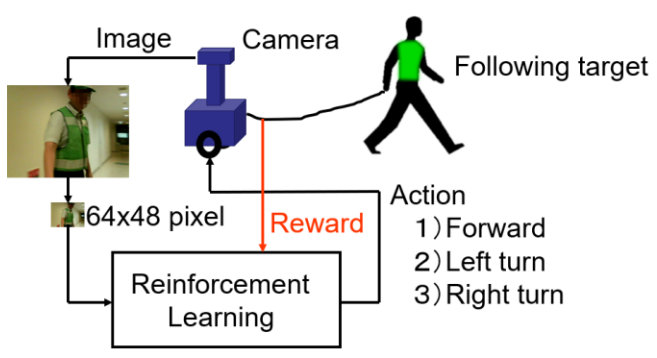
\includegraphics[keepaspectratio, scale=0.45] {images/pasin_system.png}
    \caption{Proposed method \cite{pasin1}}
    \label{Fig:pasin_system}
  \end{figure}

岡田ら\cite{okada}は,強化学習のような教師なし学習ではなく,深層学習\cite{yann2}という教師あり学習を用いて画像に基づく人追従行動を生成する手法を提案している.これは,後述するBojarskiら\cite{bojarski}の技術(end-to-end学習)を人追従問題に応用しており,強化学習を使用していないため,ロボットの行動がランダムに選択されることはない.また,学習時はルールベース制御器でロボットを制御しているので,常に人を追従する.つまり,学習時にも人追従行動を獲得することができ,強化学習を採用する手法と比べて追従対象者の負担が少ないというメリットがある.
\figref{Fig:okada_system}にシステムの概要を示す.まず,学習時は,追従対象者が引き紐を操作する.引き紐には同じくポテンショメータが取り付けられていて,ヨ―関節の変位角が0度となるようにロボットは直進や左旋回,右旋回のいずれかの行動で制御される.並行して,これらの行動とカメラ画像を深層学習器にオンラインでend-to-end学習する.学習後は,追従対象者が引き紐を操作しなくても,深層学習器によりカメラ画像を入力するだけで,出力は直進や左旋回,右旋回といった行動を選択する.つまり,学習時のルールベース制御器(引き紐による人追従行動)を模倣するように深層学習器(カメラ画像による人追従行動)は振る舞う.

  \begin{figure}[h]
    \centering
    \begin{minipage}[c]{100mm} 
        \centering
        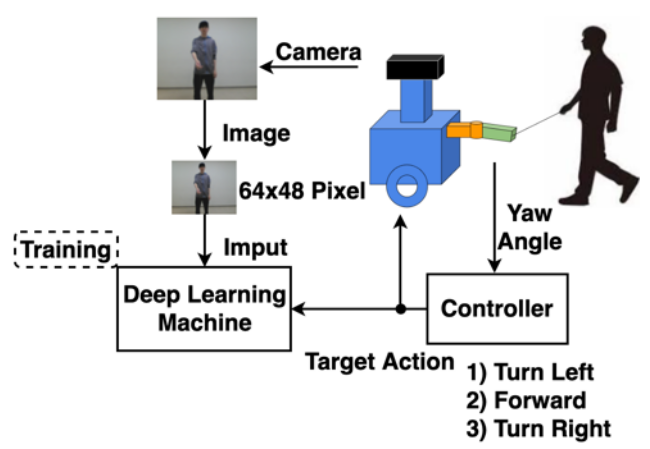
\includegraphics[width=100mm]{images/okada_learning_phase_system.png}
        \subcaption{Learning phase}
    \end{minipage} \\
    \vspace{1em} % 画像とキャプションの間にスペースを追加
    \begin{minipage}[c]{100mm} 
        \centering
        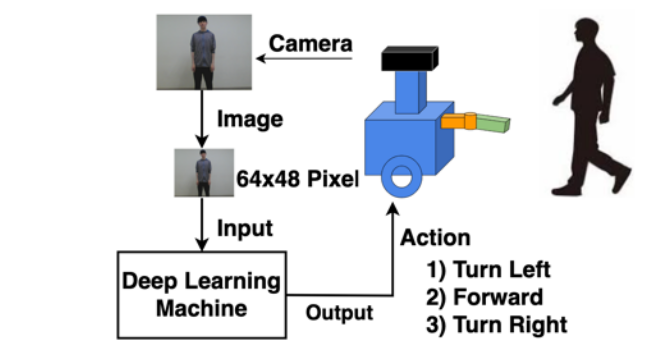
\includegraphics[width=100mm]{images/okada_following_phase_system.png}
        \subcaption{Following phase}
    \end{minipage}
    \caption{The proposed method for learning of the person-following behavior\cite{okada}}
    \label{Fig:okada_system}
  \end{figure}
% \subsection{etc...}
% \subsubsection{etc...}

\newpage

%!TEX root = ../thesis.tex

\section{関連研究}
     Bojarskiら\cite{bojarski}は,カメラ画像と人が操作するステアリングの角度を用いて模倣学習を行うことで,自動車の自動運転に成功している.学習時のシステムを\figref{Fig:bojarski_train}に示す.学習時には,ドライバーが車を運転し,その際に取得したステアリングの角度とカメラ画像を組み合わせてend-to-end学習が行われる.
     これにより,学習後は,\figref{Fig:bojarski_test}に示ようにカメラ画像から直接,ステアリングの角度を出力するシステムになっている.すなわち,カメラ画像のみで自動運転を可能にしている.
     
     \begin{figure}[h]
          \centering
          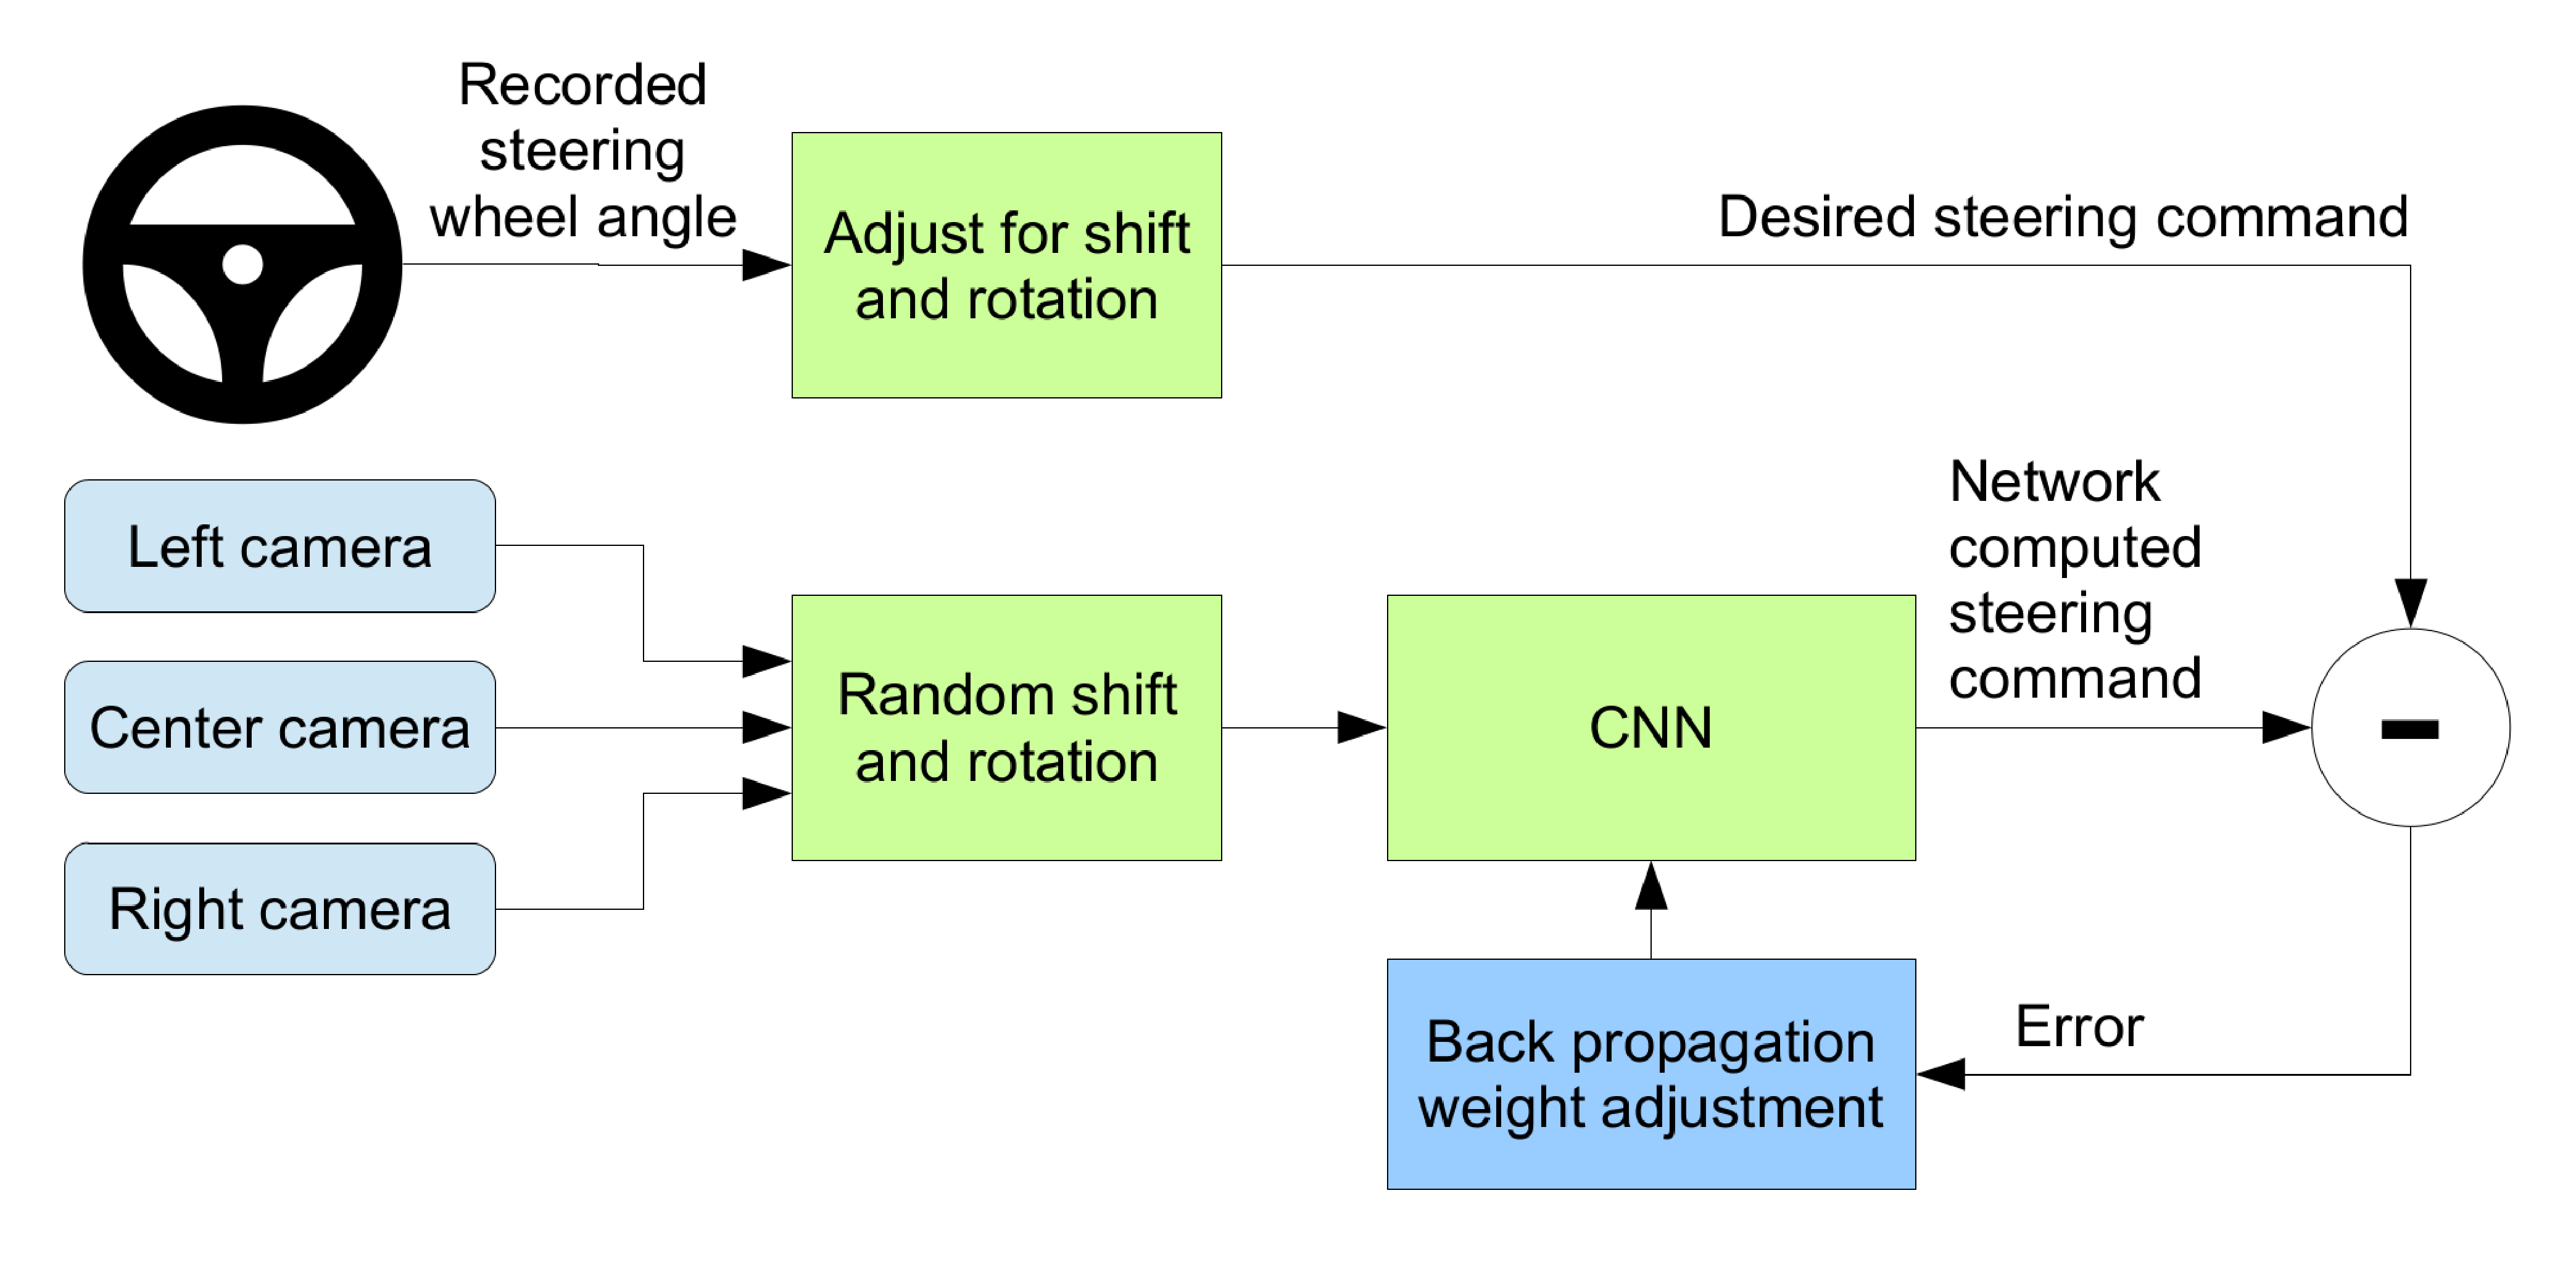
\includegraphics[keepaspectratio, scale=0.16] {images/eps/bojarski_train}
          \caption[Training the neural network]{Training the neural network (source: \cite{bojarski})}
          \label{Fig:bojarski_train}
     \end{figure}



     \begin{figure}[h]
          \centering
          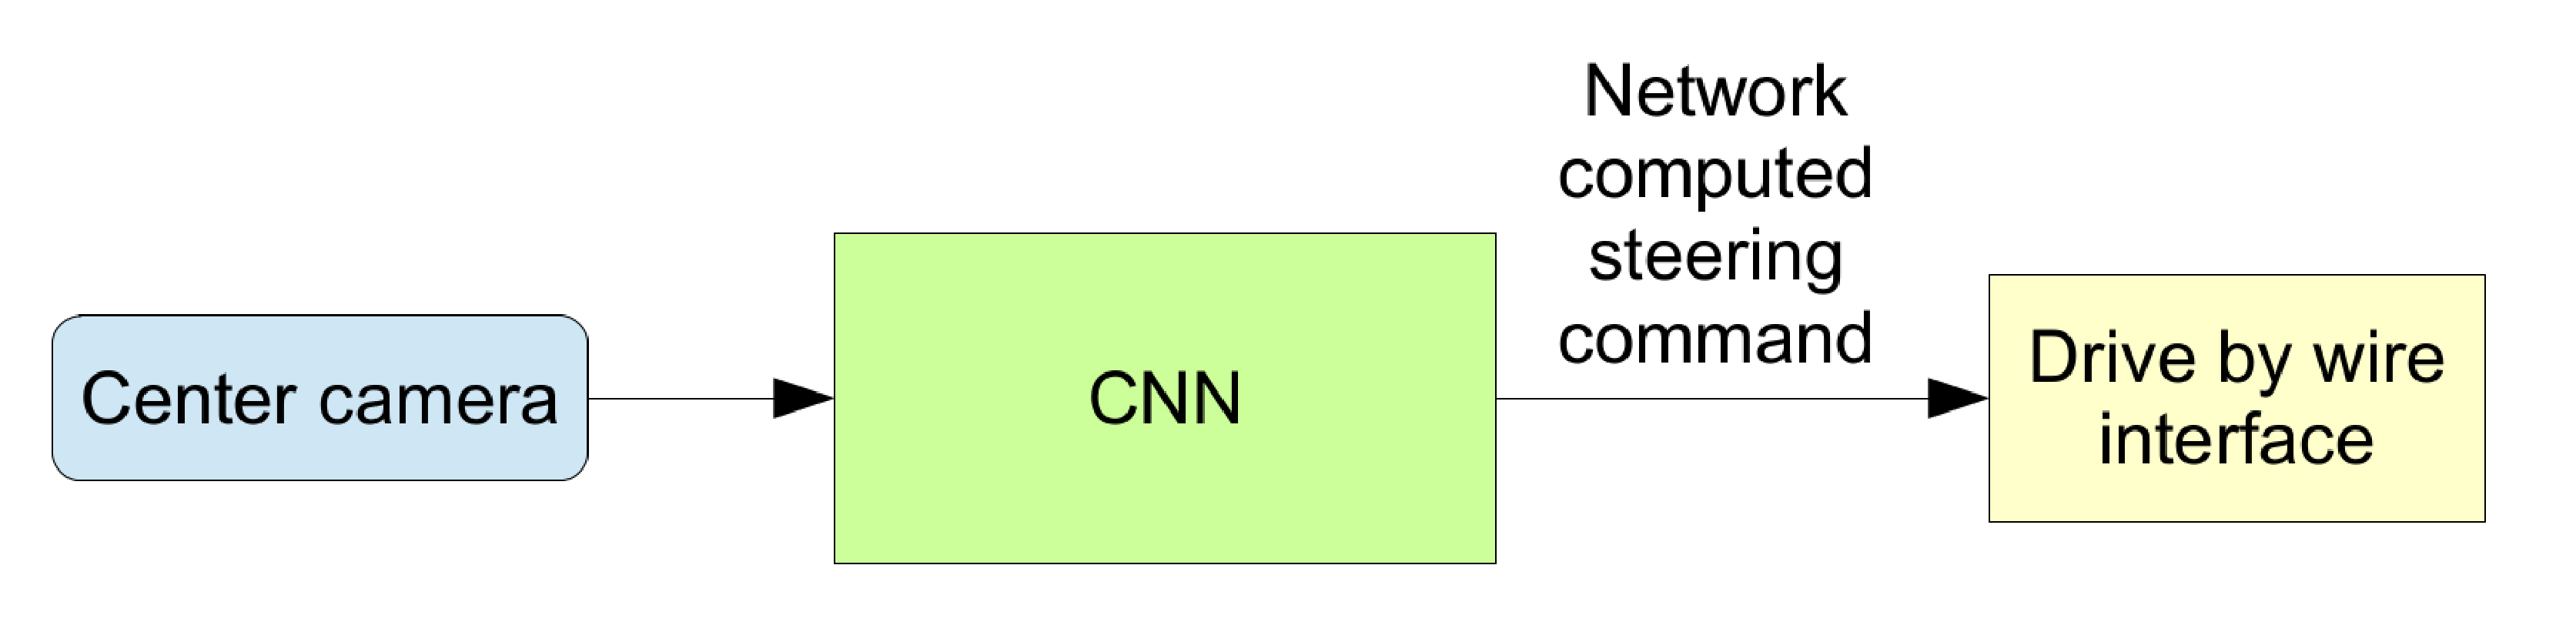
\includegraphics[keepaspectratio, scale=0.20] {images/eps/bojarski_test.eps}
          \captionsetup{justification=raggedright} % キャプションを左寄せに
          \caption[The trained network is used to generate steering commands from a single front-facing center camera.]{The trained network is used to generate steering commands from a single front-facing center camera. (source: \cite{bojarski})}
          \label{Fig:bojarski_test}
     \end{figure}

\newpage

     \figref{Fig:bojarski_CNN}は,CNNが白線等のない未塗装道路においても,人が操作するステアリングの角度だけを教師信号として用い,有用な道路の特徴を学習したことを示している.なお,道路の輪郭を検出するような学習は明示的に行っていないことが述べられている.

     \begin{figure}[h]
          \centering
          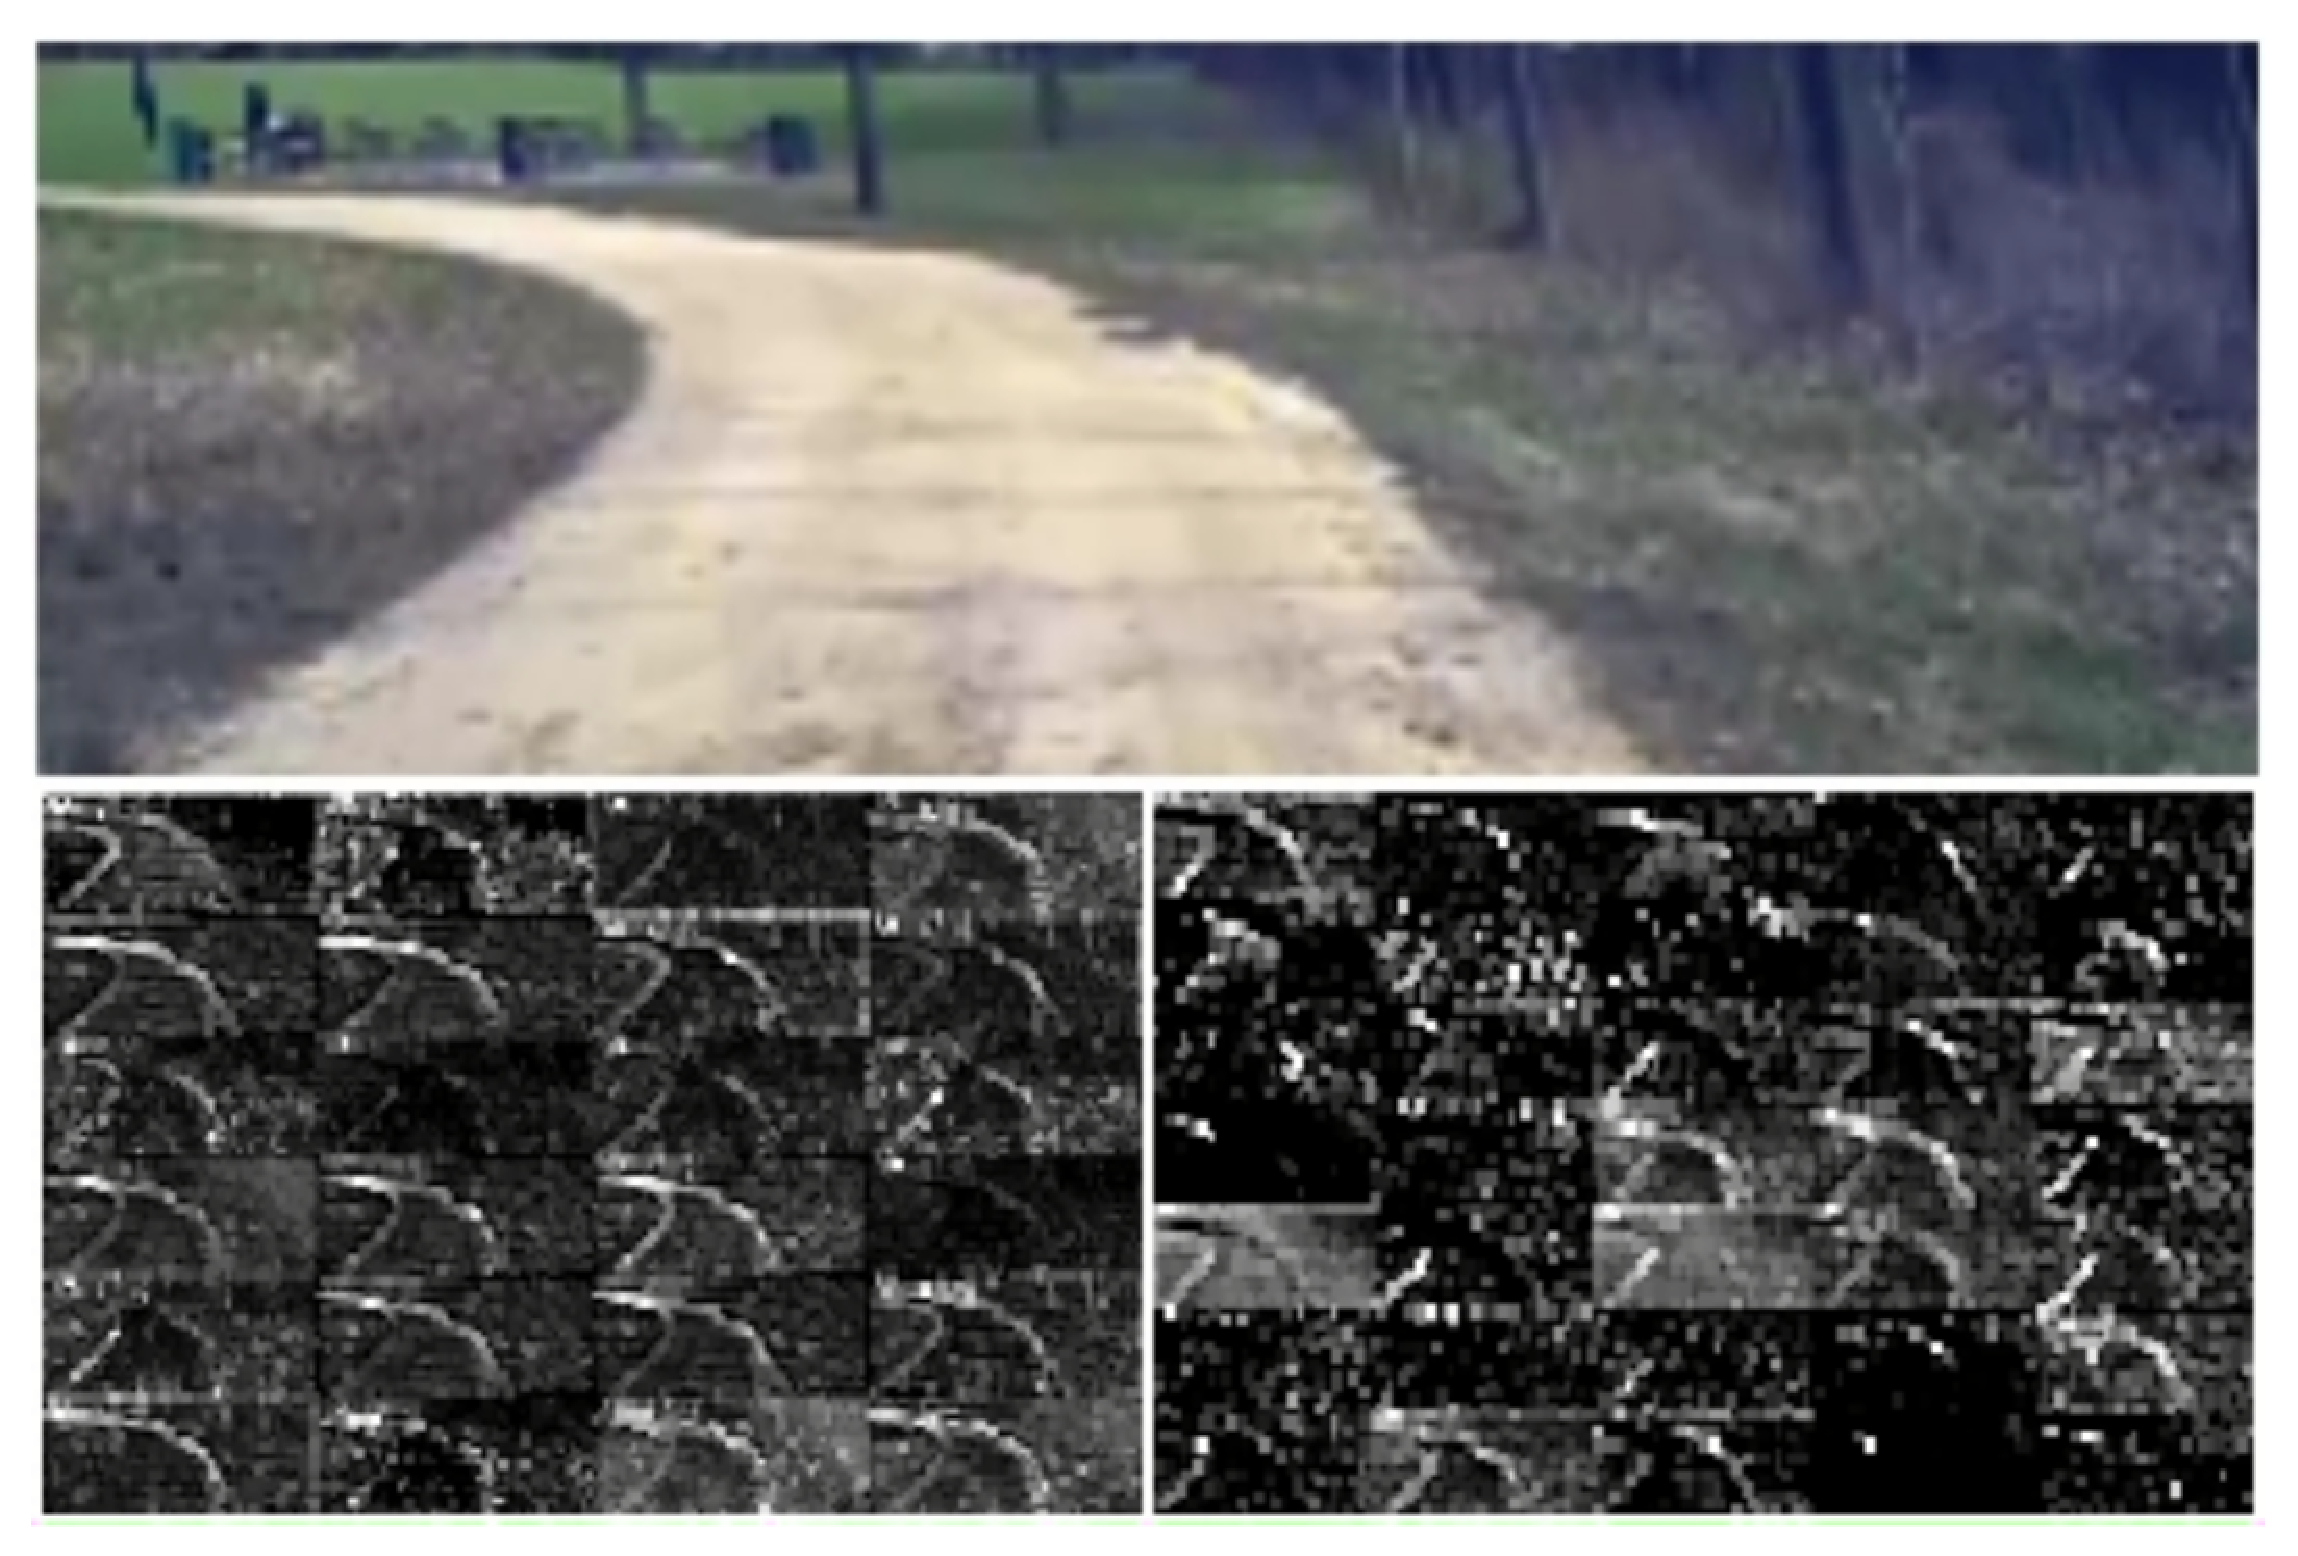
\includegraphics[keepaspectratio, scale=0.35] {images/eps/bojarski_CNN.eps}
          \captionsetup{justification=raggedright} % キャプションを左寄せに
          \caption[How the CNN ``sees'' an unpaved road. Top: subset of the camera image sent to the CNN. Bottom left: Activation of the first layer feature maps. Bottom right: Activation of the second layer feature maps. This demonstrates that the CNN learned to detect useful road features on its own, i.e., with only the human steering angle as training signal. We never explicitly trained it to detect the outlines of roads.]{How the CNN ``sees'' an unpaved road. Top: subset of the camera image sent to the CNN. Bottom left: Activation of the first layer feature maps. Bottom right: Activation of the second layer feature maps. This demonstrates that the CNN learned to detect useful road features on its own, i.e., with only the human steering angle as training signal. We never explicitly trained it to detect the outlines of roads. (source: \cite{bojarski})}
          \label{Fig:bojarski_CNN}
     \end{figure}

\newpage

%!TEX root = ../thesis.tex

\section{目的}

本研究では, 2DLiDARの反射強度を利用したルールベース制御器による人追従行動をカメラ画像を用いて end-to-end 学習して模倣する手法を提案し, カメラ画像に基づいた人追従行動が可能か, 実ロボットを用いた実験によりその有効性を検証する.

\newpage

%!TEX root = ../thesis.tex

\section{論文の構成}

  第1章では,本研究の背景,目的,関連研究について述べた.第2章では,本研究で用いる要素技術について述べる.第3章では,本研究の提案手法を述べる.第4章では,提案手法を用いた実験を行う.第5章では,本研究の結論を述べる.

\newpage

%

%ここにディレクトリのパスを追加していく
%
\chapter{マニピュレータの正しい描き方}
% \label{chap:section1}
%
%\input{introduction/preface}
%
%!TEX root = ../thesis.tex

% \section{背景}
% \subsection{RoboCup}
マニピュレータには正しい図の描き方がある.図に描いたマニピュレータの例を以下の
図 1 に示す.(a)と(b)はそれぞれ 2 自由度のマニピュレータを表しており,角度θと
長さℓの矢印以外は同じである.角度θについてはプラスとマイナスがあるため,矢印の
方向に気を付ける必要がある.よって,(b)のような矢印の描き方が望まれる.また,長
さℓについてはプラスしかないため,これも(b)のような矢印の描き方が望まれる.
\begin{figure}[hbtp]
  \centering
 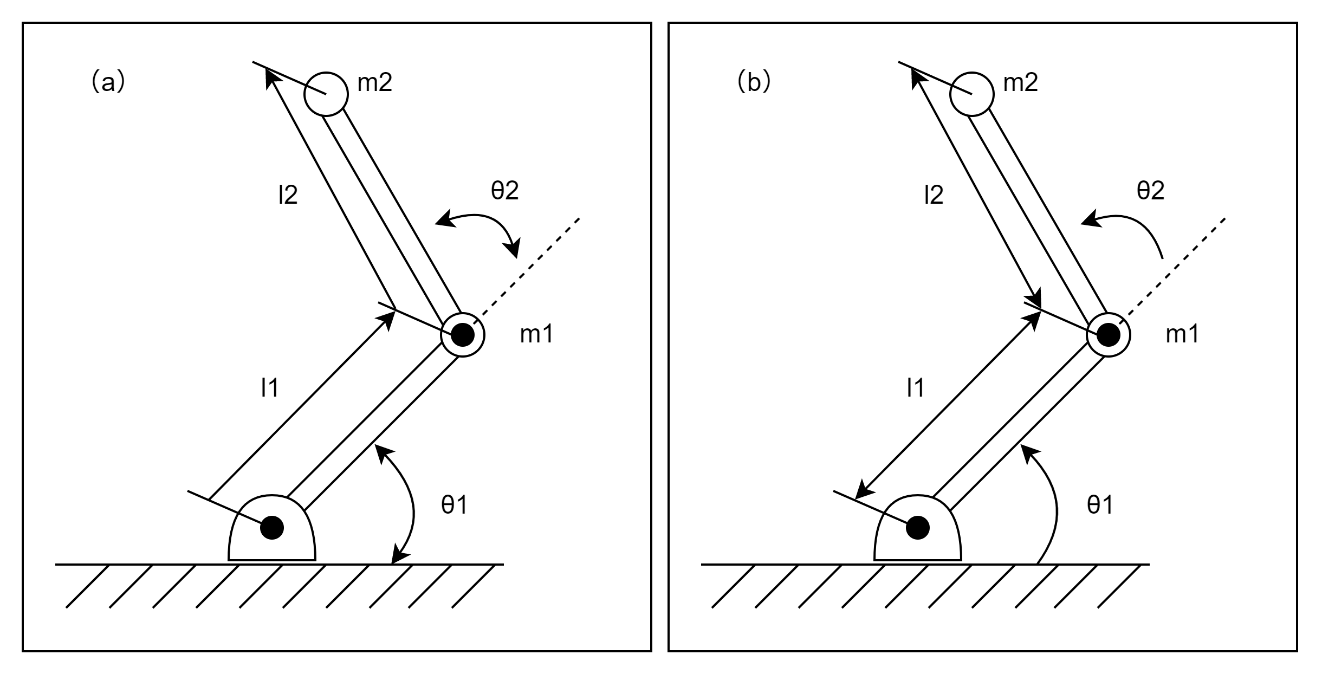
\includegraphics[keepaspectratio, scale=0.8]
      {images/mani.png}
 \caption{Manipulator}
 \label{Fig:manipulator}
\end{figure}

\newpage

%

\chapter{ラグランジュ法}

% \label{chap:section1}
%
%\input{introduction/preface}
%
 %!TEX root = ../thesis.tex

%  \section{運動エネルギ}
% \subsection{RoboCup}

% \begin{figure}[hbtp]
%   \centering
%  \includegraphics[keepaspectratio, scale=0.8]
%       {images/mani.png}
%  \caption{Manipulator}
%  \label{Fig:manipulator}
% \end{figure}
三次元空間で運動する場合,並進運動と回転運動の 2 つの成分に分けられる.並進運動
はニュートンの運動方程式,回転運動はオイラーの運動方程式で記述することができ,こ
れらを合わせてニュートン・オイラー法と呼ぶ.ニュートン・オイラー法を利用すること
で,各リンクの重心に作用する力とトルクを計算することができる.この代替手法とし
て,\textbf{ラグランジュ法}が挙げられる.ラグランジュ法は,エネルギベースのアプローチで,
剛体リンクを備えた直動マニピュレータにある程度特化している.
\newpage


 %!TEX root = ../thesis.tex

 \section{運動エネルギ}
% \subsection{RoboCup}

% \begin{figure}[hbtp]
%   \centering
%  \includegraphics[keepaspectratio, scale=0.8]
%       {images/mani.png}
%  \caption{Manipulator}
%  \label{Fig:manipulator}
% \end{figure}
マニピュレータの運動エネルギの式を定義する.$i$ 番目のリンクの運動エネルギ $k$ は,
以下の式(2.1)のように表すことができる.
\begin{equation}
     k_i= \frac{1}{2} m_i v_{Ci}^{T} v_{Ci} +\frac{1}{2} {}^{i}{\omega}_{i}^{T}  {}^{Ci} I_i {}^{i}{\omega}_i
\end{equation}
ここで,式(2.1)の第 1 項はリンクの重心の速度による運動エネルギであり,第 2 項はリンク
の角速度による運動エネルギである.マニピュレータの総運動エネルギは,個々のリンク
の運動エネルギの合計なので,
\begin{equation}
     k= \sum^{n}_{i=1}k_{i}
\end{equation}
と表すことができる.式(2.1)の $v_{Ci}$ と ${}^{i}{\omega}_{i}$ は$\theta$と$\dot{\theta}$の関数なので, マニピュレータの運動エ
ネルギは関節の位置と速度 $k(\theta,\dot{\theta})$ の関数としてスカラで記述できる.実際,マニピュレー
タの運動エネルギは次のように与えられる.
\begin{equation}
     k(\theta,\dot{\theta})= \frac{1}{2} \dot{\theta}^T M(\theta) \dot{\theta}
\end{equation}
ここで,$M(\theta)$は $n×n$ で表されるマニピュレータの質量行列である.式(2.3)の形式は,二
次関数として知られている.展開すると,結果として得られるスカラ方程式が二次関数に
依存する項のみで構成される.さらに,総運動エネルギは常に正でなければならないた
め,マニピュレータの質量行列は正定行列である必要がある.正定行列は,二次関数が常
に正のスカラであるという特性を持つ行列である.
\newpage


 %!TEX root = ../thesis.tex

 \section{位置エネルギ}
% \subsection{RoboCup}

% \begin{figure}[hbtp]
%   \centering
%  \includegraphics[keepaspectratio, scale=0.8]
%       {images/mani.png}
%  \caption{Manipulator}
%  \label{Fig:manipulator}
% \end{figure}

マニピュレータの位置エネルギの式を定義する.$i$ 番目のリンクの位置エネルギ $u_i$ は,
以下の式(2.4)のように表すことができる.
\begin{equation}
     u_i =-m_i {}^{0}g^T \; {}^{0}P_{Ci} + u_{refi}
\end{equation}
ここで, ${}^{0}g$ は $3 × 1$ の重力ベクトル,${}^{0}P_{Ci}$ は $i$ 番目のリンクの重心位置を示すベクト
ル,$u_{refi}$ は $u_i$ の最小値が得られるように選択された定数である.マニピュレータに保存
される位置エネルギの合計は,個々のリンクの位置エネルギの合計なので,
\begin{equation}
     u= \sum^{n}_{i=1}u_{i}
\end{equation}
と表すことができる.式(2.4)の ${}^{0}P_{Ci}$は$\theta$の関数なので,マニピュレータの位置エネルギは関
節位置$u(\theta)$の関数としてスカラで記述できる.
\newpage


 %!TEX root = ../thesis.tex

 \section{ラグランジュ}
% \subsection{RoboCup}

% \begin{figure}[hbtp]
%   \centering
%  \includegraphics[keepaspectratio, scale=0.8]
%       {images/mani.png}
%  \caption{Manipulator}
%  \label{Fig:manipulator}
% \end{figure}

動的なラグランジュの定式では,機械システムの運動エネルギと位置エネルギの差とし
て定義されるラグランジュと呼ばれるスカラ関数から方程式を導き出す手段を提供してい
る.マニピュレータのラグランジュを式で表すと以下の式(2.6)のようになる.
\begin{equation}
     {\cal L}(\theta,\dot{\theta})= k(\theta,\dot{\theta})-u(\theta)
\end{equation}
マニピュレータの運動方程式は以下の式(2.7)のようになる.
\begin{equation}
     \frac{d}{dt}\frac{\partial\cal L}{\partial\dot\theta}-\frac{\partial\cal L}{\partial\theta}=\tau
\end{equation}
ここで $\tau$ はアクチュエータのトルクで $n × 1$ ベクトルである.マニピュレータの場合,この
方程式は,
\begin{equation}
     \frac{d}{dt}\frac{\partial k}{\partial\dot\theta}-\frac{\partial k}{\partial\theta}+\frac{\partial u}{\partial\theta}=\tau
\end{equation}
のように $k(∙)$ と $u(∙)$ の引数は簡潔のため省略される.
\newpage


%

%% Back Matter
\backmatter{}
%
\chapter{提案手法}

  本章では,従来手法をベースとする提案手法の概要,提案手法における学習フェーズ,追従フェーズ,ルールベース制御器,ネットワーク構造についての5節に分けて述べる.

\label{chap:suggest}
%
%!TEX root = ../thesis.tex

\section{提案手法の概要}

  本研究は,ルールベース制御器の入力に引き紐ではなく,2DLiDARの反射強度を利用する.このときのロボットの行動を\figref{Fig:RobotGuidance_velocity}に示す.並進速度は,学習時と学習後で共に0.2 \,[m/s]で一定であり,ロボットのヨ―方向の角速度$\omega$のみが変化する.ルールベース制御器は,反射強度の高い方向にロボットを追従させる制御で,追従対象者に再帰反射テープを装着し,2DLiDARでそれを検出することで,人に追従する手法である.

  \begin{figure}[h]
    \centering
    \begin{minipage}[c]{65mm} 
        \centering
        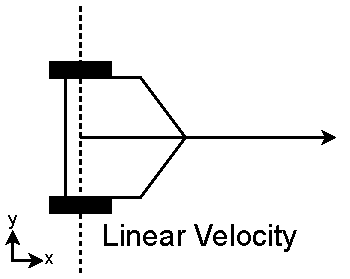
\includegraphics[height=40mm]{images/pdf/RobotGuidance_linear_velocity}
        \subcaption{Forward is fixed}
    \end{minipage}
    \begin{minipage}[c]{65mm} 
        \centering
        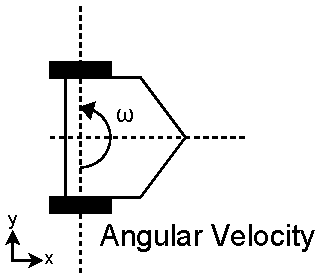
\includegraphics[height=40mm]{images/pdf/RobotGuidance_angular_velocity}
        \subcaption{Angular velocity changes depending on input}
    \end{minipage}
    \caption{Output robot actions}
    \label{Fig:RobotGuidance_velocity}
  \end{figure}

\newpage

  深層学習器は,ルールベース制御器の出力(ロボットのヨ―方向の角速度$\omega$)とRGB画像をend-to-end学習することで,\figref{Fig:RobotGuidance_simple_system}に示すように,入力をRGB画像,出力をロボットのヨ―方向の角速度$\omega$として人を追従する.

  \begin{figure}[h]
    \centering
    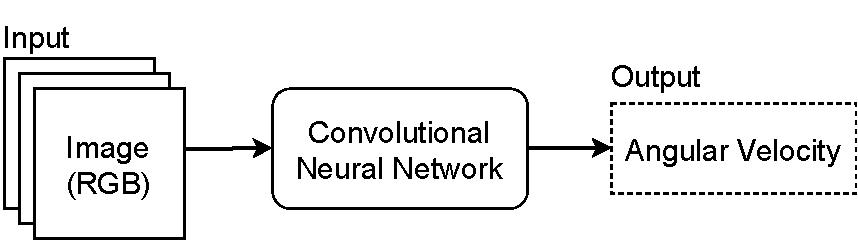
\includegraphics[height=3cm] {images/pdf/RobotGuidance_simple_system}
    \captionsetup{justification=raggedright} % キャプションを左寄せに
    \caption{The trained network is used to generate the robot's yaw angular velocity from the RGB images}
    \label{Fig:RobotGuidance_simple_system}
  \end{figure}

  \figref{Fig:RobotGuidance_all_system}に示すように,ルールベース制御器を用いてロボットを制御するフェーズを学習フェーズ,深層学習器の出力をロボットの行動にするフェーズをテストフェーズと呼ぶこととする.以下に,学習フェーズとテストフェーズの主な役割を示す.

  \subsubsection*{<学習フェーズ>}
  2DLiDARの反射強度を利用したルールベース制御器に従い,ロボットを制御する.制御器の出力と画像を教師信号として深層学習器に与え,オンラインでend-to-end学習する.
  
  \subsubsection*{<テストフェーズ>}
  2DLiDARは使用せず,画像を入力とした深層学習器の出力をロボットの行動にする.画像に基づいた人追従ができるかを実験により確認する.

  \begin{figure}[h]
    \centering
    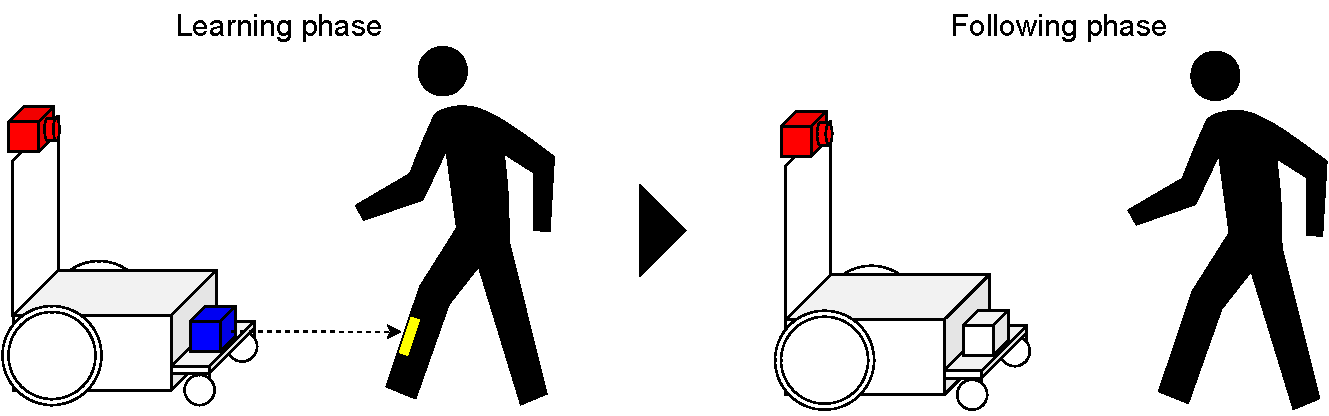
\includegraphics[height=3.5cm] {images/pdf/RobotGuidance_all_system}
    \captionsetup{justification=raggedright} % キャプションを左寄せに
    \caption{Sequence of proposed method}
    \label{Fig:RobotGuidance_all_system}
  \end{figure}

\newpage

%!TEX root = ../thesis.tex

\section{学習フェーズ}

  学習フェーズの概要を\figref{Fig:RobotGuidance_learning_system}に示す.学習フェーズでは,2DLiDARの反射強度を利用したルールベース制御器を用いて,\figref{Fig:RobotGuidance_learning_phase_leg}に示す追従対象者の足に装着した再帰反射テープに向かって,ロボットを制御する.ルールベース制御器の出力は,ロボットのヨ―方向の角速度$\omega$の1つとし,角速度$\omega$が0 \,[rad/s]となるようにロボットを制御することで人追従することが可能と考えられる.並行して,この行動とカメラの画像データを深層学習器に入力して,オンラインで学習させる.なお,並進速度は0.2 \,[m/s]で一定にしているため,深層学習器に入力しない.

  \begin{figure}[h]
    \centering
    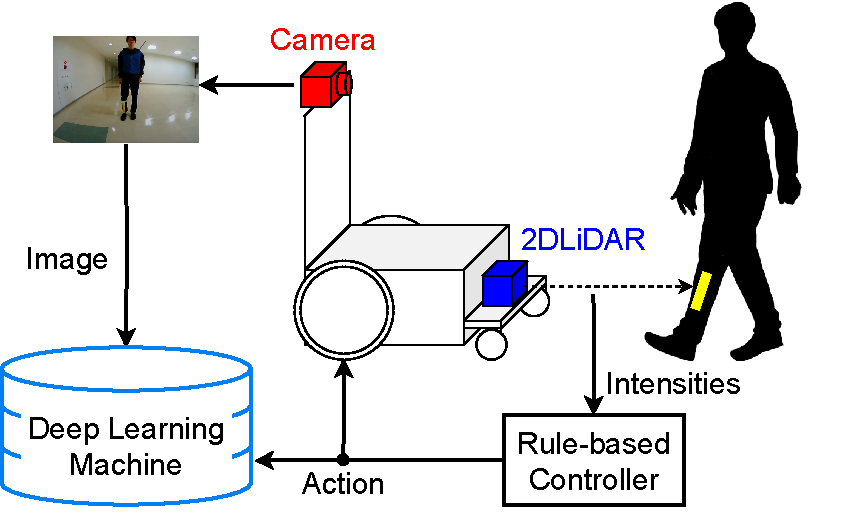
\includegraphics[keepaspectratio, scale=0.45] {images/pdf/RobotGuidance_learning_system}
    \captionsetup{justification=raggedright} % キャプションを左寄せに
    \caption{Proposed method in the learning phase}
    \label{Fig:RobotGuidance_learning_system}
  \end{figure}

  \begin{figure}[h]
    \centering
    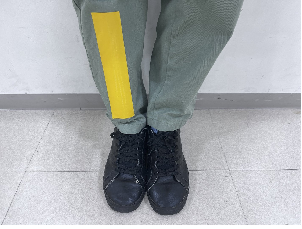
\includegraphics[keepaspectratio, scale=0.55] {images/pdf/RobotGuidance_learning_phase_leg}
    \captionsetup{justification=raggedright} % キャプションを左寄せに
    \caption{Wearing retroreflective tape}
    \label{Fig:RobotGuidance_learning_phase_leg}
  \end{figure}

\newpage

%!TEX root = ../thesis.tex

\section{追従フェーズ}

  追従フェーズの概要を\figref{Fig:RobotGuidance_following_system}に示す.追従フェーズでは,学習フェーズで獲得したモデルを用いる.ここでは,2DLiDARを使用せず,代わりに深層学習器の出力がロボットの行動に影響を与える.つまり,2DLiDARの反射強度に基づくルールベース制御器の出力ではなく,画像を入力とした深層学習器の出力がロボットの行動を決定する.

  \vspace{0.5cm}

  \begin{figure}[h]
    \centering
    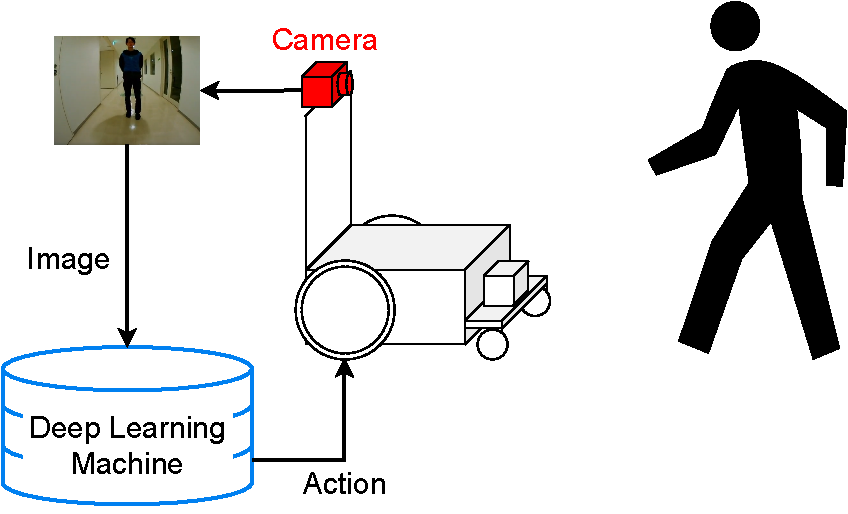
\includegraphics[keepaspectratio, scale=0.45] {images/pdf/RobotGuidance_test_system}
    \captionsetup{justification=raggedright} % キャプションを左寄せに
    \caption{Proposed method in the test phase}
    \label{Fig:RobotGuidance_following_system}
  \end{figure}

  \vspace{0.5cm}

  \begin{figure}[h]
    \centering
    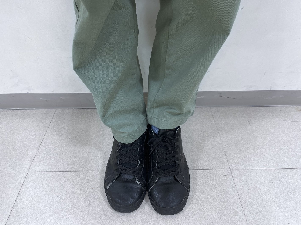
\includegraphics[keepaspectratio, scale=0.55] {images/pdf/RobotGuidance_test_phase_leg}
    \captionsetup{justification=raggedright} % キャプションを左寄せに
    \caption{Without retroreflective tape}
    \label{Fig:RobotGuidance_following_phase_leg}
  \end{figure}

\newpage

%!TEX root = ../thesis.tex

\section{反射強度を計測する装置}

  本研究で使用した2DLiDARは北陽電機社製のUTM-30LX\cite{hokuyo}である.このセンサは,ROS上で提供されている\texttt{urg\_node}\cite{urg_node}というパッケージを使用することでデータの取得ができる.この2DLiDARは,物体までの距離情報だけでなく,物体の反射強度の値も取得可能である.基本的には,\texttt{urg\_node}で提供されているデフォルトのパラメータを使用するが,\tabref{tab:parameters_of_urg_node}に示すように一部のパラメータを変更している.このセンサ自体の最大検出範囲は270 \,[deg]であるが,反射強度モードを使用する際には最大検出範囲を120 \,[deg]に制限することが推奨されている\cite{urg_node}.そのため,センサの正面を0 \,[deg]としたときに,左側に60 \,[deg](1.047 \,[rad]),右側に-60 \,[deg](-1.047 \,[rad])とした.また,1回のスキャンは25 \,[ms]時間がかかり,-60 \,[deg]から0 \,[deg]を通り60 \,[deg]に向かってレーザが回転する.この動作を\figref{Fig:Image of scan}に示す.

  \begin{table}[hbtp]
    \caption{Parameters of \texttt{urg\_node}}
    \label{tab:parameters_of_urg_node}
    \centering
    \begin{tabular}{c|cc}
    \hline
    Parameter name & Default & Experiment \\ 
    \hline
    \hline
    intensities & false   & true         \\ 
    angle\_min  & -       & -1.047       \\ 
    angle\_max  & -       & 1.047        \\ 
    \hline
    \end{tabular}
    \end{table}

    \vspace{-0.5cm}

    \begin{figure}[h]
      \centering
      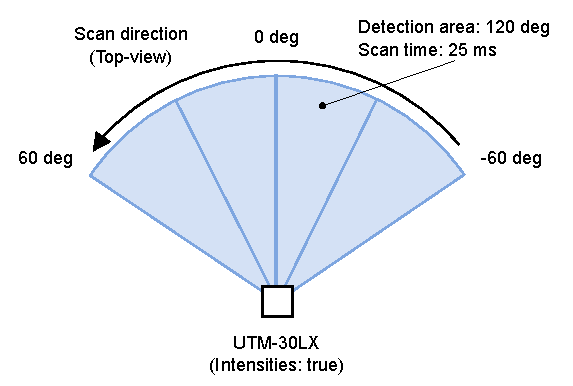
\includegraphics[height=5.5cm] {images/pdf/RobotGuidance_hokuyo_scan}
      \captionsetup{justification=raggedright} % キャプションを左寄せに
      \caption{Condition of scan}
      \label{Fig:Image of scan}
    \end{figure}

\newpage
%!TEX root = ../thesis.tex

\section{ルールベース制御器}

  学習フェーズで使用するルールベース制御器は,前節で述べた2DLiDARの反射強度を利用しており,最大反射強度の方にロボットが追従する手法となっている.この制御器の出力は,ロボットのヨ―方向の角速度$\omega$の1つであり,角速度$\omega$が0 \,[rad/s] となるようにロボットを制御する.角速度$\omega$は,以下の式\eqref{eq:angular_velocity}で表され,角度に応じた角速度$\omega$が式\eqref{eq:inequality}の範囲で出力される.

  \begin{equation}
    \omega[\text{rad/s}] = \frac{1}{\theta_{\text{max}}} \times \theta
    \label{eq:angular_velocity}
    \end{equation}

  \begin{equation}
    1 \geq \omega \geq -1
    \label{eq:inequality}
    \end{equation}

  ルールベース制御器からの出力を\tabref{tab:output_from_rule-based_controllers}に示す.ここでは,わかりやすくするために行動を左旋回,直進,右旋回の3つに分解しているが,実際に出力される行動はロボットのヨ―方向の角速度$\omega$の1つであることに注意する.

  \begin{table}[h]
    \caption{Output from rule-based controllers}
    \label{tab:output_from_rule-based_controllers}
    \begin{tabular}{|c|c|c|c|}
    \hline
    Action & Control rule {[}rad{]} & Linear velocity {[}m/s{]} & Angular velocity {[}rad/s{]} \\ 
    \hline
    Turn Left & $\text{angle\_max} \geq \theta > 0$ & 0.2 & $1 \geq \omega > 0$ \\ 
    \hline
    Forward & $0$ & 0.2 & $0$ \\ 
    \hline
    Turn Right & $0 < \theta \leq \text{angle\_min}$ & 0.2 & $0 > \omega \geq -1$ \\ 
    \hline
    \end{tabular}
    \end{table}

\newpage

  ルールベース制御器によるロボットの行動を\figref{Fig:RobotGuidance_learning_turn_left}と\figref{Fig:RobotGuidance_learning_turn_right}に示す.これは,RVizで部分的に可視化したもので,右足に装着した再帰反射テープに反応し,最大反射強度として周辺の色(黄色)とは異なる色(紫色)で表示している.
  
  \figref{Fig:RobotGuidance_learning_turn_left}の(a)は,2DLiDARの左前方にいる人(再帰反射テープ)を検出し,その角度に応じた角速度$\omega$の値が出力され,左旋回する.その結果,(b)のように角速度$\omega$はほぼ0 \,[rad/s]に近づき,直進する.

  \figref{Fig:RobotGuidance_learning_turn_right}の(a)は,2DLiDARの右前方にいる人(再帰反射テープ)を検出し,その角度に応じた角速度$\omega$の値が出力され,右旋回する.その結果,(b)のように角速度$\omega$はほぼ0 \,[rad/s]に近づき,直進する.

\begin{figure}[h]
  \centering
  \begin{minipage}[c]{65mm} 
      \centering
      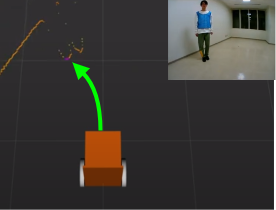
\includegraphics[height=40mm]{images/RobotGuidance_learning_turn_left_(a).png}
      \subcaption{Turn left}
  \end{minipage}
  \begin{minipage}[c]{65mm} 
      \centering
      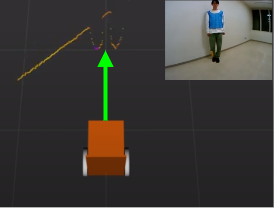
\includegraphics[height=40mm]{images/RobotGuidance_learning_turn_left_(b).png}
      \subcaption{Forward}
  \end{minipage}
  \caption{Turn left toward the retroreflective tape}
  \label{Fig:RobotGuidance_learning_turn_left}
\end{figure}

\begin{figure}[h]
  \centering
  \begin{minipage}[c]{65mm} 
      \centering
      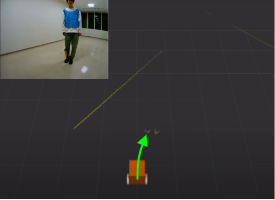
\includegraphics[height=40mm]{images/RobotGuidance_learning_turn_right_(a).png}
      \subcaption{Turn right}
  \end{minipage}
  \begin{minipage}[c]{65mm} 
      \centering
      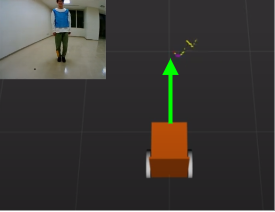
\includegraphics[height=40mm]{images/RobotGuidance_learning_turn_right_(b).png}
      \subcaption{Forward}
  \end{minipage}
  \caption{Turn right toward the retroreflective tape}
  \label{Fig:RobotGuidance_learning_turn_right}
\end{figure}

\newpage

%!TEX root = ../thesis.tex

\section{ネットワーク構造}

  ネットワークを\figref{Fig:RobotGuidance_network}に示す.これは,深層学習フレームワークであるPyTorch\cite{pytorch}を使用し,CNNをベースとしている.具体的には,入力層,畳み込み層3,全結合層2,出力層の7層で構成している.深層学習器は,縮小された画像と選択された行動を0.2秒周期で収集して学習する.これを1stepとする.使用したハイパーパラメータを\tabref{tab:Parameters of network configured with pytorch}に示す.

  \begin{figure}[h]
    \centering
    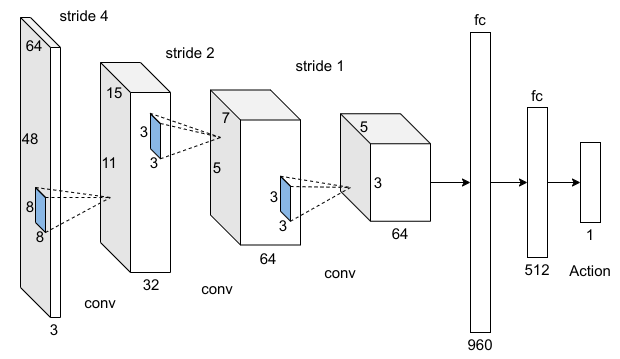
\includegraphics[keepaspectratio, scale=0.60] {images/RobotGuidance_network.png}
    \caption{Architecture of the network}
    \label{Fig:RobotGuidance_network}
  \end{figure}

  \begin{table}[hbtp]
    \caption{Parameters of network configured with PyTorch}
    \label{tab:Parameters of network configured with pytorch}
    \centering
    \begin{tabular}{cc}
      \hline
      Input data & Image(64x48 pixels, RGB channels) \\
      Optimizer & Adam($alpha = 0.001, beta1 = 0.9, beta2 =  0.999, eps = 1e^{-2}$)\\
      Loss function & Softmax-cross-entropy\\
      Output data & Angular velocity\\
      \hline
    \end{tabular}
  \end{table}

\newpage


%

%

\end{document}
